      
\documentclass[a4paper,11pt]{kth-mag}

\usepackage[acronym]{glossaries}
\glsdisablehyper
\usepackage{textcomp}
\usepackage[table]{xcolor}
\usepackage[hidelinks]{hyperref}
\usepackage{todonotes}
\usepackage{lmodern}
\usepackage{amsmath}
\usepackage{amsthm}
\usepackage{url}
\usepackage[swedish,english]{babel}
\usepackage{modifications}
\usepackage{multirow}
\usepackage{textcomp}
\usepackage{listings}
\usepackage{color}
\usepackage{amssymb}
\usepackage{dirtree}
\usepackage{array}
\usepackage{pdfpages}
\usepackage{longtable}
\usepackage[acronym]{glossaries} 
\usepackage{graphicx} %To use pictures
\usepackage[T1]{fontenc} %Includes '>'
\usepackage[utf8]{inputenc} %för åäö


\graphicspath{ {images/} }







%\usepackage{comment} % enables the use of multi-line comments (\ifx \fi) 
%\usepackage{fullpage} % changes the margin



\makeglossaries
\setlength\parindent{0pt}

\extrafloats{1000}
\bibliographystyle{ieeetran}
\title{Title goes here}
\subtitle{Thesis WIP}
\foreigntitle{Title in Swedish goes here}
\author{Richard Odell}
\date{\today}
\blurb{Master's Thesis at ITM\\Supervisor: Lars Svensson \\ Examiner: Lei Feng}
\trita{TRITA xxx yyyy-nn}


\newacronym{rcv}{RCV}{Research Concept Vehicle}
\newacronym{mpc}{MPC}{Model Predictive Controller}
\newacronym{itrl}{ITRL}{Integrated Transport Research Lab}
\newacronym{pi}{PI}{Proportional-Integral}
\newacronym{abs}{ABS}{Anti-lock Braking System}
\newacronym{dc}{DC}{Direct Current}
\newacronym{pid}{PID}{Proportional-Integral-Derivative}
\newacronym{kth}{KTH}{The Royal Institute of Technology}
\newacronym{mbd}{MBD}{Model-Based Design}





\begin{document}

\frontmatter
\pagestyle{empty}
\removepagenumbers
\maketitle
\selectlanguage{english}


\clearpage
\begin{abstract}

Write the abstract here.

\end{abstract}
\clearpage
\begin{foreignabstract}{swedish}
Abstract in Swedish goes here.

\end{foreignabstract}
\clearpage

\chapter*{Acknowledgements}

I would like to thank...



\glsaddall
\printglossary
\renewcommand{\glsnamefont}[1]{\textbf{#1}}
\printglossary[type=\acronymtype,style=super,nonumberlist,nopostdot,nogroupskip]


\clearpage
\clearpage
\tableofcontents*
\clearpage
\listoffigures*
\clearpage
\listoftables*
\glsaddall



\mainmatter
\pagestyle{newchap}

%%%%%%%%%%%%%%%%  INTRODUCTION   %%%%%%%%%%%%%%%%%%%%%%%

\chapter{Introduction}

This chapter will give an introduction to the thesis. 

\section{Background}
The \gls{rcv} is a platform for research in vehicle autonomy and vehicle dynamics at \gls{kth}. It is an electric vehicle with four electric hub motors at each wheel. The vehicle has room for two persons, one driver and one passenger, and it can be driven both manually as well as autonomously. For precise autonomous operation, accurate actuation of steering input and wheel torque is critical. The electrical wheel motors of the \gls{rcv} can produce torque for acceleration and braking up to a limit. However, for hard braking maneuvers, regenerative braking is not sufficient and a hydraulic brake system actuated by electric linear actuators is used in addition. In the original configuration, the hydraulic brakes actuate fairly slow (>1s before braking request is met). Thus, a redesign of the control software and the mechanical assembly is needed. The task is challenging due to the non-linear and environment dependent dynamics of the hydraulic system.

\section{Purpose}
The vehicle industry as well as industry in general is moving towards automation to lower costs, risks, lead times and work load for employees. Today there already exists some form of autonomous driving in vehicles, such as Tesla's Auto pilot and Volvo which are conducting tests with autonomous highway driving around Gothenburg. For the technology to be accepted by the masses it need to be safe and not put people, property or environment at risk. Since the \gls{rcv} is built for autonomous driving, but lacks an efficient friction brake, the purpose of this thesis will be to evaluate and improve the performance of the friction brake system. The updated braking system on the \gls{rcv} will be discussed how they can be applied in general autonomous vehicles, 

To fulfil the purpose a couple of research questions was set up. These are 
\begin{itemize}
\item Which are the most common methods used in friction brake controllers in brake-by-wire systems and autonomous vehicles? 
\item How does the chosen control method enhance how the torque request are met, compared to the original hardware setup and controller?
\item Can the controllers achieve an error of a maximum of 5\% of the requested torque at all times?
\end{itemize}

\section{Delimitations}
A lot of aspects affects the behavior of the brakes, and  achieving a properly functioning brake with good reaction time will consume much time. Therefore delimitations must be made in order to make the thesis feasible within the limited time frame. The focus of this thesis will be on making an existing braking system faster in terms of reaction time of reaching the requested braking torque. 

Wheel slip and \gls{abs} are both important factors while designing a modern brake, but this will not be implemented or considered in this thesis due to the fact that there is simply not enough time. Split mu, meaning when there is different friction coefficients acting on the the wheels, for example when one wheel travels over a slip of ice or gravel, will not be considered either. The parts that has been left out will be seen as future work that can be made to further improve the brakes on the vehicle. 

 
\section{Research design/Methodology}
The methodology used for this project will be a case study of how to implement one or more brake controllers, which works best for solving the problem stated together with a comparison of the controllers advantages and disadvantages. The case study will have its focus on qualitative research, as there's extensive work already done within this area. The testing will also have a quantitative orientation in the end to validate the brake model as well as how the controller performs. 

\subsection{Tests}
To evaluate the results of this thesis, tests will be made to compare how the system behaves with the old hardware and controller compared to the new system setup. The first type of test will consist of the \gls{rcv} standing still and then giving different torque requests of 5, 10, 20 and 40 Bar, five iterations for each pressure level, and then measuring the response time by plotting the results. 
The other test will be testing the braking performance in terms of braking distance. These tests was done at test track 2 at Arlanda. Tests was done with the help of Lars Svensson driving the \gls{rcv} and getting it up to speed, and at a certain point marked with traffic cones, brake the vehicle as hard as possible by requesting a predetermined torque from the mechanical brakes. The brake test was done at two different speeds, 15 and 30 km/h, for both the old setup and the new, three tests was done for each test case. 


\section{Ethics}
A reliable braking systems is one of the most vital functions to the safety of a vehicle. Without functioning brakes a vehicle can easily become a death trap for both people inside the vehicle as well as people in the immediate surroundings. 
Although this project will be designing the braking system from an autonomous point of view, i.e. the braking will ultimately be controlled by a computer, there will still always be one or two people in the car monitoring the autonomous driving, whom might be susceptible to great risks if the brakes do not work. To keep risks at acceptable levels there is a manual brake pedal that can override the autonomous drive mode braking, and brakes the vehicle if necessary. This brake pedal is controlled by the person in the drivers seat, who shall have experience with the vehicle and is aware of the risks and behaviour of the car. 

The vehicle is not legal to drive in regular traffic, and thus it is only driven in big closed off areas, such as a runway on Arlanda or in a closed off parking lot, where it is driven at low speeds of up to 45 km/h. The vehicle is also equipped with seat belts dimensioned for racing. 
Since the \gls{rcv} has an electric propulsion system, the people close to the vehicle will not be exposed to any harmful exhausts gases. 


\section{Risk assessment}
The risks that is involved with this project concerns mainly the availability of the \gls{rcv} and that if new parts are needed that they get delivered on time. Since new parts can have rather long lead times, if they are not off the shelf items, they need to be ordered as soon as possible to not hold up the whole project. Concerning the availability of the \gls{rcv}, which is shared amongst many different projects, is that tests that are needed can be planned and executed without disturbing other students. If any mechanical work needs to be done to the vehicle, this needs to be planned as well, firstly to be sure that the vehicle is available and secondly so that it doesn't interfere with other tests or demonstrations etc.. 
Anther risk is that conducting most tests on the vehicle requires two persons, one which will be driving the vehicle and one that controls the computer that will be running the test. Since the test phase and later parts of the thesis takes place during late summer, the planned tests need to take vacations of key people in the project into account. \newline

%%%%%%%%%% I will probably skip this part?
%\section{Requirements?}
%
%- Speed of the actuators, in ms before request to actual torque meet.
%
%- Should it be optimized for torque meet, or regeneration? that is, should the regenerative me used as torquefill or as main brake? Probably torque fill.
%
%- Maximum negative acceleration / deceleration.
%
%%%%%%%%%%%

\section{Outline}
What does the report discuss?
This chapter discusses this, this other chapter discusses that...

To be filled in later when most of chapters is done.


%%%%%%%%%%%%%%%%%   BACKGROUND STUDY   %%%%%%%%%%%%%%%%

\chapter{Background study}
To be able to answer the questions of this thesis and to base the thesis on fact a literature study was made. The study includes information about the hardware setup, both which are preferably used in state of the art as well as information about the parts already mounted on the \gls{rcv}, together with information about controllers used for controlling the system. This chapter presents the background study that was conducted together with conclusions draw by the study.


\section{Frame of reference}
The literature search began with searches in the IEEE Xplore database, but ended up using Google Scholar as the main search engine for articles, papers and reports that was of value to this thesis. The search began with broad definitions such as 'braking system autonomous driving' as well as 'braking control methods in autonomous driving' trying to get reports that included everything in the braking system, such as the hardware as well as software and controllers. As stated before the main idea in the beginning was to just make a new controller to the brakes on the \gls{rcv}, but this was broadened to also include the implementation of new hardware. This resulted in that the background study had to be oriented towards hardware as well. 

The literature searches showed that there where a few methods of controlling a brake actuator or braking system that appeared more frequently than other. These methods where then included in the search, together with searches solely for that method. This way each search only resulted in a few certain articles or papers where most of them where relevant or at least semi-relevant to this thesis project. These articles and their contents are discussed in the following sections withing this chapter.



\subsection{Braking systems for autonomous vehicles}
Yu et al. \cite{Yu} discusses differences in a linearly actuated system vs a hydraulic pump system. The linearly actuated system uses a linear actuator that press directly on a hydraulic cylinder, while a hydraulic pump system uses an electric pump to build up pressure and controls the pressure in the system by valves and/or solenoids. The linear actuators are simpler and more fail safe, since it doesn't have as many valves from where there can be a leakage of hydraulic fluid. 


\vspace{5mm}
Line, Manzie and Good \cite{4475522} has constructed a electro-mechanical  brake-by-wire system, which utilizes an electrical motor in the calipers as actuator that controls the pressure between the brake pads and the rotor. There is also a brake pedal that sense the pedal position which in turn sends the brake request to a controller. They compare two different controllers in this paper, a cascaded \gls{pi} controller and a \gls{mpc}. The cascaded \gls{pi} controller has three control loops for force, motor angular velocity and motor current. The \gls{pi} controller works, but due to the systems nonlinearity it is somewhat inconsistent in different situations. The \gls{mpc} performs better in this case, but in order for it to work this efficiently a very good model of the system is needed as ground work, and this is time consuming. \newline


Xiang et al. \cite{Xiang} writes that a electro-mechanical system is preferable over a electro-hydraulical system, due to the simplicity, the efficiency and stability, the enhanced diagnostic capabilities, cost reduction, space and weight saving as well as the elimination of environmental concerns associated with traditional hydraulic braking systems.\newline

%\vspace{5mm}
Line, Manzie and Good \cite{2004-01-2050} as well as in Ahn et al. \cite{ahn2009analysis} are articles about using a cascaded \gls{pi} controller to control a electro-mechanical brake-by-wire system. Here they present requirements on a electromechanical braking system. They discuss the influence of friction, which makes the system nonlinear. The nonlinearity is discussed in the conclusion, where the nonlinear system is the explanation why the cascaded pi controller does not work as fast in the lower brake pad force spectrum as it does for the higher part of the spectrum. \newline



Frede, Khodabakhshian and Malmquist \cite{Frede460614} has written a state-of-the-art report on by-wire systems, with an extensive part about brake-by-wire. They present an overview of brake blending strategies as well as control strategies to regulate braking torque. Most reports discuss brake blending control, but reports where  brake torque control is achieved by fuzzy logic is presented as well. Isermann \cite{661149} also describes the strengths of a fuzzy logic controller, due to its ability to handle nonlinear systems. \newline

Milan{\'e}s et al. \cite{milanes2010electro} presents in an article how an autonomous braking system is implemented into a ordinary road car. The car is already fitted with a hydraulic braking system with a manually controlled braking pedal, and the autonomous braking system is added on to that, resulting in a electro-hydraulic autonomous braking system similar to that on the \gls{rcv}. 
Although the actuator in this car is a electric pump compared to a linear actuator on the \gls{rcv}, this report shows that a electro-hydraulic system is satisfactory, even though other reports state that electro-mechanical systems are preferable \cite{MechatronicsBook} \cite{Xiang}. \newline

The brake blending will be done by a simple function where the regenerative brakes brakes as much as possible, and when they have reached their maximum braking power, the friction brakes steps in to fill in the missing torque, as described by Troung \cite{truongdevelopment}. \newline

\section{Linear actuators}
something about linear actuators
\section{Controllers}
Something about PID controllers and other common actuators.
\section{Results/Conclusions from background study}
The results from the literature study is that the two friction brake controllers will consist of a \gls{pid} controller and a fuzzy logic controller. 
The brake blending algorithm will be a simple one where the regenerative brakes brake as much as possible, and the friction brakes fills in the missing torque. 


%%%%%%%%%%%%%%%%%%   IMPLEMENTATION   %%%%%%%%%%%%%%%

\chapter{Implementation}

This chapter presents how the braking system is implemented by creating a model of it in Simulink using Simscape and describes the tuning of the controller. Information about the original system is presented, as well as why and how new actuators where implemented and used by the friction brake system. New mounts had to be designed and produced as well to fit the new actuators, and this process is presented too. \\

% Describe how measuremets of stopping distance was made? No, this was done in Method section. 


\section{Original setup/system hardware setup}
The friction braking system that was used in the \gls{rcv} is a electro hydraulic braking system. The braking system is made up of two linear actuators which are controlled by current from a driver, which in turn get its signal from a dSpace controller, the main computer in the \gls{rcv}. The linear actuators acts on hydraulic cylinders that transfers the force to the calipers on each wheel, where the force acts on the rotors which brakes the vehicle. The reason there are two linear actuators is due to the fact that there are two completely separated friction braking systems in the vehicle, one system that acts on the two front wheels, and the other that acts on the two rear wheels. This is done to incorporate a higher level of safety, whereas if one of the systems breaks down, there will still be braking abilities on two of the four wheels. \newline

There is also a manually operated braking pedal that acts on the hydraulic system, controlling the brakes on all four wheels. This braking pedal which is mechanically connected directly to two hydraulic cylinders is located between the calipers and the hydraulic cylinders connected to the linear actuators. If the manual brake pedal is pressed, the autonomous braking system is mechanically disconnected, and all braking is controlled by the driver. \newline

[Picture of brake system setup]

\section{Brake actuators and new mounts}
At the start of this thesis project the plan was to use the original hardware setup that existed in the \gls{rcv}. However, it was soon realised that the actuators together with how they were assembled was a large limiting factor in the speed of the braking system. A decision was made to change to a new set of actuators that are both faster as well as stronger. New actuators led to the mounts required a re-design because of the different form factor of compared to the old actuators. 

\subsection{Original actuators and lever arm}
The original actuators, named Electrak 1, was of an acme screw type, which involves a lot of dynamic friction where up to 80\% of the input power is dissipated in friction losses [SOURCE]. This means that the motor within the actuator has to work hard to move the rod in each direction. The static friction is also very high, which raises a problem when it come to the control of the actuator. The actuator requires a high current to start moving to overcome the static friction, and when it has overcome that static friction the need of current to keep the motion going is not as high. Thus, the steps in current that is needed to make the actuator move offers a problem in controlling it, since it is hard to control with the step in current that is needed and very small movements in the actuator rod can have large effects to the pressure of the hydraulic system. \\

However, one feature that could be useful in the acme leadscrew actuators is that the configuration is, within certain forces, self locking. They function in such a way that it moves easily if force is applied from one direction , while if it is applied in the other direction it has to be very high in order for the piston to move. Thus, they can be used as parking brake when the vehicle is turned of, if no other means of parking brake is present. Since the ballscrew actuator has lower internal friction, it cannot be relied upon as parking brake. Though, a parking brake can easily be realized by other means, such as a lever  connected to the manual parking brake etc., and is therefore not included in the scope of this thesis\\

The hardware setup, in terms of mounts and lever arm, that was originally mounted on the \gls{rcv} needed revision as well, especially the lever arms that transferred the force from the actuator to the hydraulic cylinder. As can be seen in picture [SOURCE TO PICTURE], there is a lever arm that transfers the force from actuator to hydraulic cylinder. This arm is over dimensioned, the lever arm is to long. Tests showed that the acme screw actuators reaches their stroke limit when the request for braking torque reaches a certain point, which means that the actuators is able to provide higher force than  originally is possible, hence, the lever arms can be shortened in order to make the system faster while keeping the amount of force that can be delivered. 

\subsection{New actuators}
New actuators was needed to make the system faster, characteristics such as low internal friction and fast linear motion speed are desirable. Concerning the friction, a change from acme screw to ball screw actuators had to be made since ball screw actuators incorporate drastically lower friction then an acme screw [SOURCE?MAYBE??]. \gls{itrl} has good contacts with Thomson Linear, which is a large linear motion supplier in Sweden, a decision was made to order one of their actuators due to decent lead times and prices, as well as the possibility of invoicing. Thomson Linear offers many different ball screw actuators, but the decision fell on the Max Jac with a maximum force of 800 Newton and a speed of 30 millimeters per second at full load. Compared to the old actuators, the Electrak 1, which has a maximum force of 225 Newton and a speed of 33 millimeters per second at full load, the new one are much stronger, albeit slightly slower at full load. What is interesting though, is not the speed at full load, but the no-load speed since the brake actuation in the beginning requires little force but high speeds, which is 60 millimeters per second for the Max Jac and only 45 millimeters per second for the Electrak 1. The datasheet of the Max Jac can be found in appendix \ref{appendix:Max_Jac} and the datasheet of the Electrak 1 can be found in appendix \ref{appendix:Electrak_1}.\\

To be sure that the new actuator can deliver enough force, the maximum braking force for the whole vehicle must be calculated. The highest needed braking torque on each wheel was calculated with respect to the maximum negative acceleration that is stated in the requirements. If the acceleration is known, as well as the mass of the vehicle the total force that needs to act on the vehicle can be calculated with Newtons second law, 
\begin{equation}
F_{tot}=m\cdot a,
\end{equation}
where $F_{tot}$ is the total force needed to achieve acceptable deceleration, $m$ is the mass of the vehicle and $a$ is the acceleration. The vehicle has four wheels and the force is considered to be divided evenly distributed on each wheel. Hence, this gives us 
\begin{equation}
F_{wheel}=\frac{F_{tot}}{4},
\end{equation}
where $F_{wheel}$ is the force needed on each wheel. The torque needed on that wheel can then be calculated by 
\begin{equation}
M=F_{wheel}\cdot r,
\end{equation}
where $M$ is the torque and $r$ is the radius of the wheel. The required torque on each wheel was calculated to 350 Nm.\\

The step from torque to pressure in hydraulic system was made earlier when the original braking system was implemented, before this thesis started. It was done by a series of tests where the electric motors where set to give a specific torque and the brakes where actuated manually to meet that torque by letting the \gls{rcv} move slightly, and then note the pressure in the hydraulic system for that torque. The result was linear,and thus the pressure can be multiplied by a constant to get the applied braking torque. If the maximum braking torque needed is 350 Nm, we get a maximum pressure of 15.4 Bar in the hydraulic system.


\subsection{Mounts for new actuators}

During this thesis a decision was made to change the original actuators to a pair of new ones with different dimensions. The new actuators was of ball screw type, which incorporate lower friction, both static and dynamic. This will help a lot when constructing the controller for the brakes, since we won't have as high step in the current needed to start moving the actuator rod. \\

New mounts had to be made to fit the new actuators, which are slightly larger than the original lead screw actuators. These mounts where modeled in the 3D CAD program Solid Edge, and can be seen in Figure \ref{fig:CAD_Actuator_mount} and Figure \ref{fig:CAD_Hydraulic_cylinder_mount}. These parts where then manufactured by water jet cutting by the machine design department at \gls{kth}. The parts that were constructed were new mounts to the actuators, mounts to the hydraulic cylinders as well as a new connection between the actuator and lever arm. The hydraulic cylinders has not been changed during the thesis project, but since the actuator mounts has been made wider as the actuators are wider, the cylinders had to be wider apart as well to get everything to line up properly. \\

The connection between the actuator and lever arm was made with regards to the possibility to change the position of the connection on the lever arm, to be able to change the leverage. The connection consists of a T-shaped part that is mounted on the actuator while also clamping on to the lever arm with the help of another piece of metal with holes drilled, two screws and bolts. \\

\begin{figure}[h]
\centering
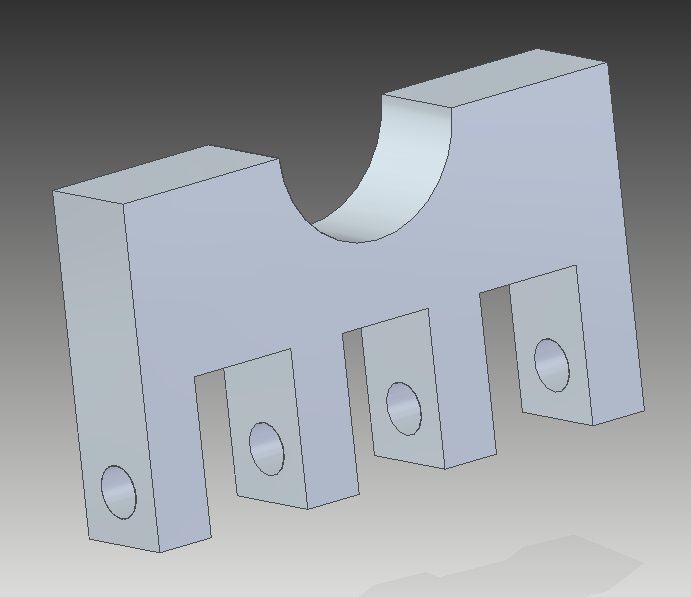
\includegraphics[width=0.5\textwidth]{Actuator_mount}
\caption{CAD picture of mount}
\label{fig:CAD_Actuator_mount}
\end{figure}

\begin{figure}[h]
\centering
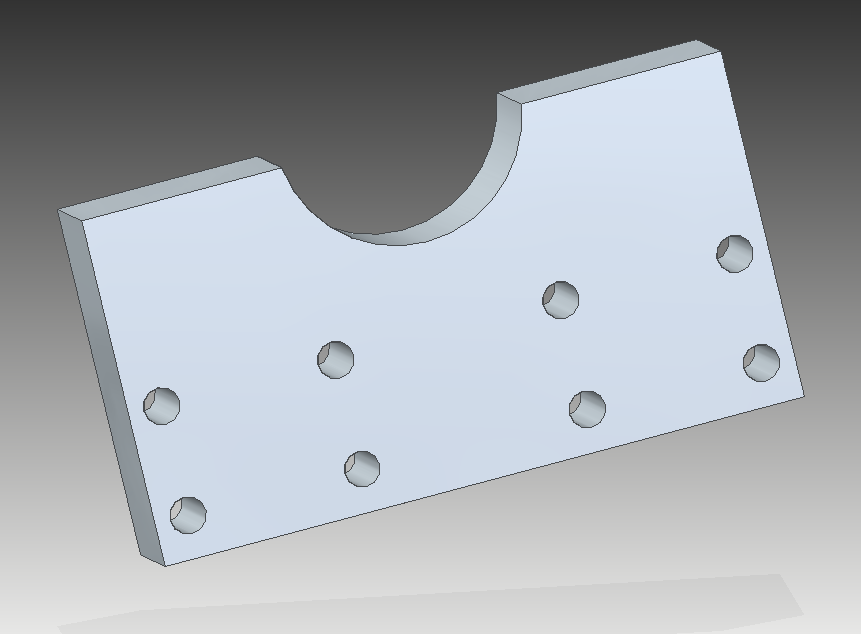
\includegraphics[width=0.5\textwidth]{Hydraulic_cylinder_mount}
\caption{CAD picture of the hydraulic cylinder mount}
\label{fig:CAD_Hydraulic_cylinder_mount}
\end{figure}



\section{Implementation and tuning in simulink/simscape}

The development of the controller was made using \gls{mbd}, where the model was made using the graphical programming environment Simulink. Primarily the tool box Simscape was used, which is a tool box useful while designing physical systems. The model was then VERIFIED, and used while tuning the brake controller. 

\subsection{Simscape model and \gls{mbd}}
The plant model was constructed in Simulink, mostly using the Simscape toolbox. The plant is made up of a few different parts which are the hydraulic system, the brake calipers, electric actuators and mechanical force translation such as lever arm. All of these parts are made up of Simscape blocks that are tuned by either measured or calculated values as well as values derived from data sheets. The Max Jac linear actuator is made up of three primary internal components, which are the electric \gls{dc} motor, a gear box and the ball screw. To acquire all the constants of the motor, the gearing of the sprockets and ball screw one of the actuators where dismantled, and all necessary parts were measured and calculated to get all required information. 

Information concerning the hydraulic system, exact information has been difficult to acquire due to the fact that it is mounted on the vehicle and practically impossible to remove just for measurements, due to the fact that it is used daily by other students and researchers, and would take too much time to dismount, measure and then mount again. No datasheets or drawings was to be found either. Therefore some measurements was made on the outside of the calipers, and an inner volume of the cylinder and diameter of the piston was then estimated upon those measurements. For the master cylinder the measurements is more exact due to the fact that there were a spare cylinder in the workshop that measurements could be done upon. The lever arms where measured while still mounted on the vehicle as well. \\

The choice of using \gls{mbd} was due to the fact that it is an easy and fast. This way of solving a problem by making a software plant model and designing the controller from there is called \gls{mbd}, which has become a very popular method of solving engineering problems, since when a plant model has been made it is easy, fast and cheap to develop and improve the controls\cite{2010-01-1999}. 

\subsection{Verification of simscape model}
When the complete model in Simulink was done it needed to be verified before tuning of the controller could be done. The verification was made by running the physical system with the new actuators and all necessary hardware mounted at certain current requests and then compare the results with from the same cases of current request on the plant model. The results can be seen in [FIGURE]. \\



The verification was done at certains currents fed into the actuators, these where 500, 800, 1000 and 1500 mA. This corresponded to 12, 35, 48 and 68 Bar. While running the system will not go above 20 Bar, but because of the internal coulomb friction the actuator did not move until about 400-500 mA where applied, these levels were used to verify the model.\\

When the rear brakes were applied the pressure sank in the front, which means the system in not that exact, and is why the verification can be accepted. \\

No way to implement coulomb friction, which is a big part in these acme and lead screws. This is (probably) why the validation becomes sort of bad.\\



\subsection{Tuning controller}
An attempt was made to tune the \gls{pi}-controller using pole placement. The braking system model was linearised at around 2 Bar, and then the system was linearized to a second order transfer function. This simplified system was then used when tuning the controller using pole placement. However, after several tries with poles placed in different locations in the left half plane, no useful results had been acquired. 

Since the tuning of the controller with the help of pole placement did not give any useful values, this method was abandoned, and instead a trial and error method was used in the existing \gls{pi}-controller. Values on \begin{math} K_{p}\end{math} and \begin{math} K_{i} \end{math} was based on the values that worked for the original design with the old actuators.\\ 


The values that was deemed best during the tests at Arlanda was \begin{math} K_{p}=50,K_i=10 \end{math}. The original controller included a feed forward part, which was tuned to  \begin{math} FF = 60 \end{math}. 
An anti wind-up function was implemented in the \gls{rcv} main simulink model from the start, and no changes was made to this function, since no evidence of wind-up did occur during tuning. \\


%%%%%%%%%%%%%   RESULTS   %%%%%%%%%%%%%%%%%%%%


\chapter{Results}
This chapter presents the results from the tests that was made in this thesis.

\section{Actuator response time}
This section will show the plots of tests while \gls{rcv} standing still. 

\section{Brake distances}
This section presents result from brake distance tests. Figure \ref{fig:New_15kph_test1} to \ref{fig:Old_30kph_test3} shows plots of braking tests with both new and old actuators from 15 and 30 km/h. 
The braking distance from Figure \ref{fig:New_15kph_test1} to \ref{fig:Old_30kph_test3} is compiled in to Table \ref{tab:table1}.


\begin{figure}[h]
\centering
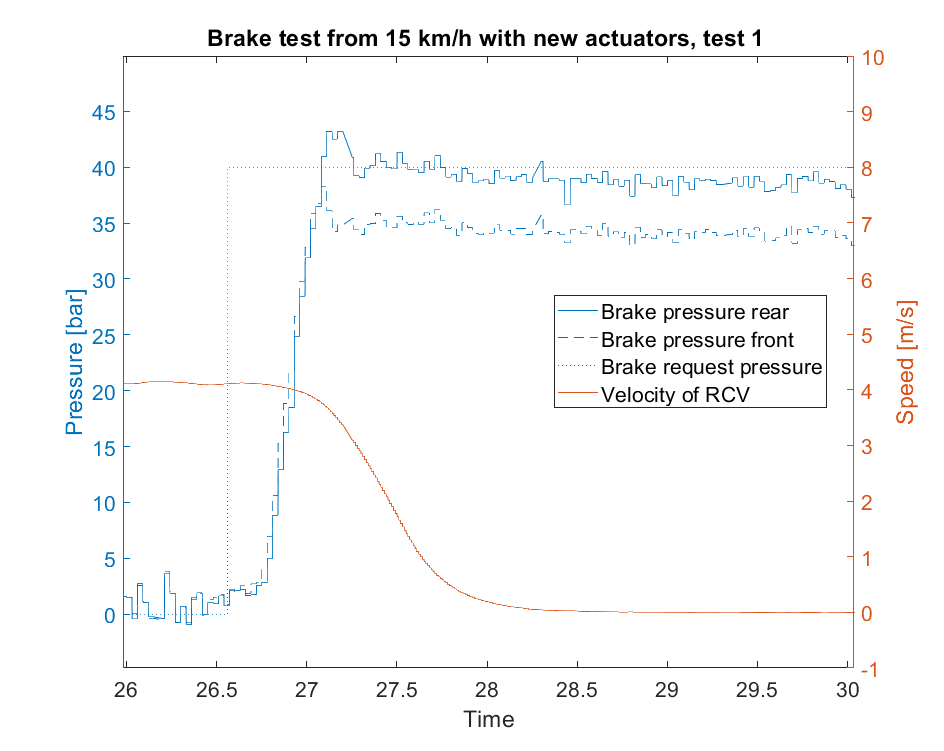
\includegraphics[width=0.8\textwidth]{New_15kph_test1}
\caption{New actuator, 15 km/h, test 1}
\label{fig:New_15kph_test1}
\end{figure}

\begin{figure}[h]
\centering
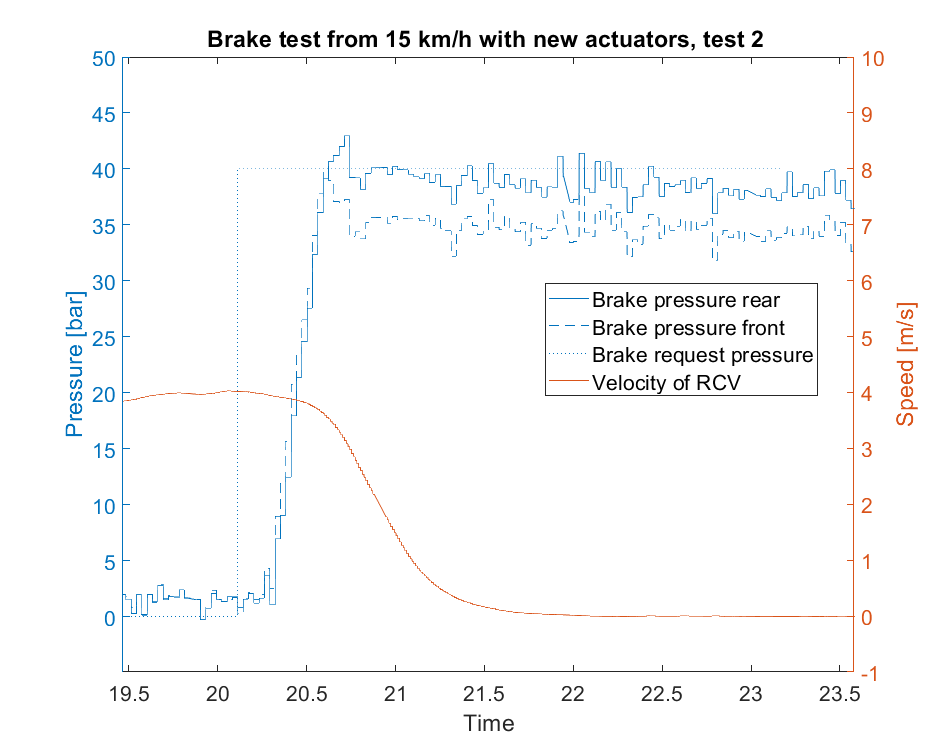
\includegraphics[width=0.8\textwidth]{New_15kph_test2}
\caption{New actuator, 15 km/h, test 2}
\label{fig:New_15kph_test2}
\end{figure}

\begin{figure}[h]
\centering
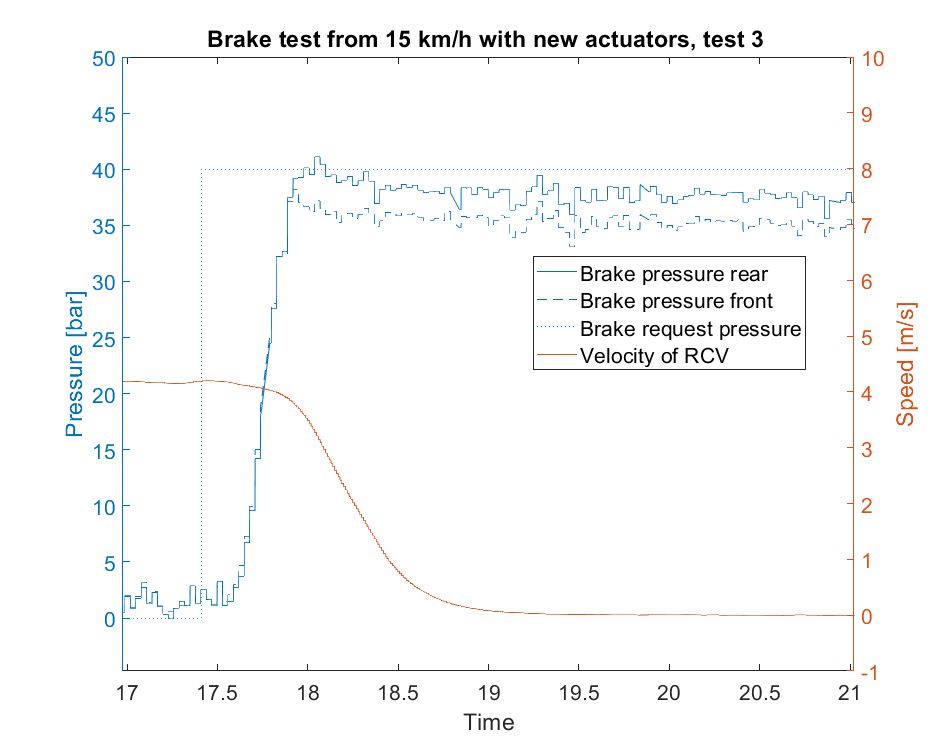
\includegraphics[width=0.8\textwidth]{New_15kph_test3}
\caption{New actuator, 15 km/h, test 3}
\label{fig:New_15kph_test3}
\end{figure}

\begin{figure}[h]
\centering
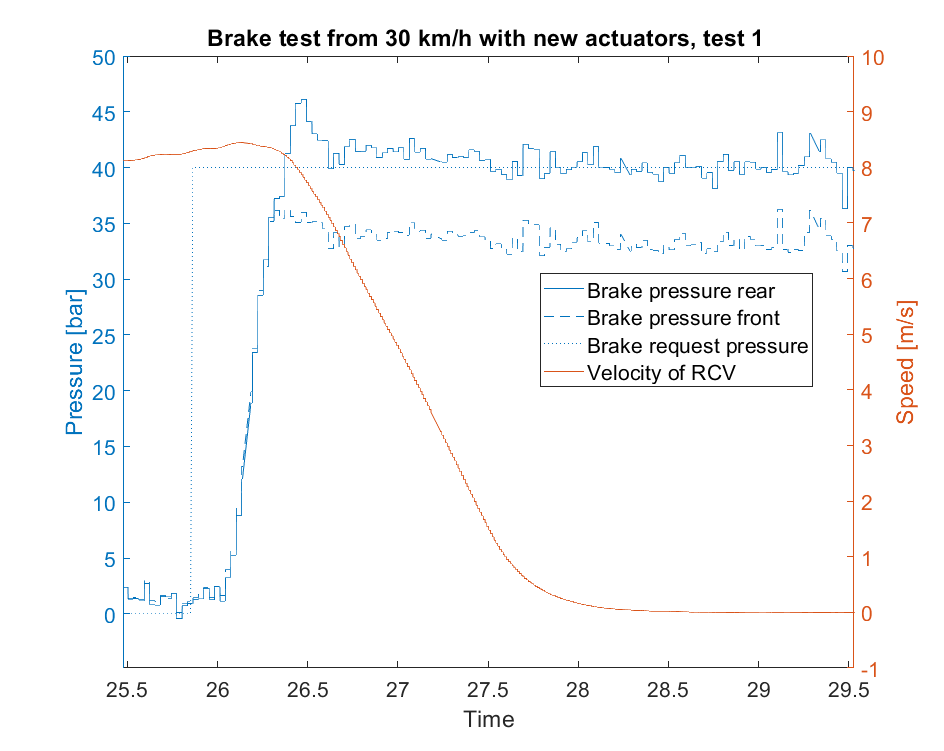
\includegraphics[width=0.8\textwidth]{New_30kph_test1}
\caption{New actuator, 30 km/h, test 1}
\label{fig:New_30kph_test1}
\end{figure}

\begin{figure}[h]
\centering
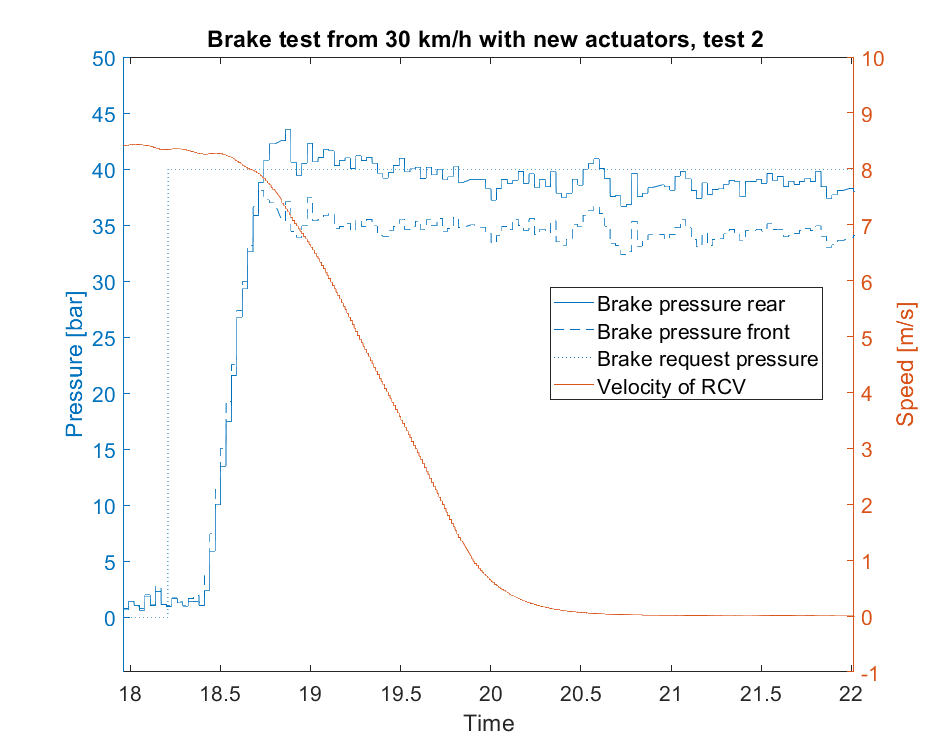
\includegraphics[width=0.8\textwidth]{New_30kph_test2}
\caption{New actuator, 30 km/h, test 2}
\label{fig:New_30kph_test2}
\end{figure}

\begin{figure}[h]
\centering
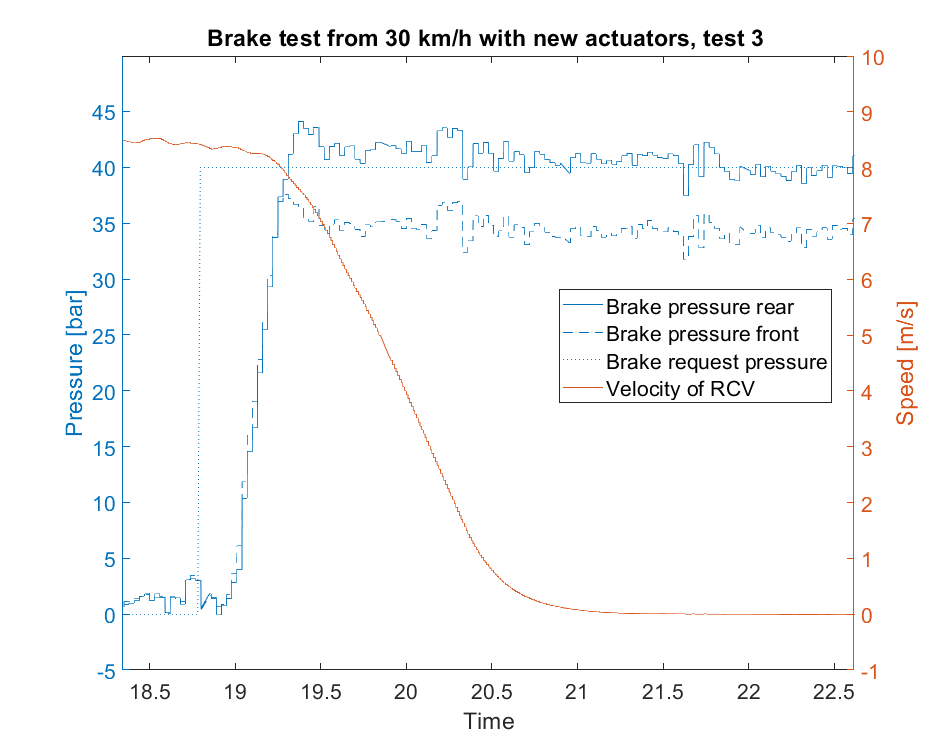
\includegraphics[width=0.8\textwidth]{New_30kph_test3}
\caption{New actuator, 30 km/h, test 3}
\label{fig:New_30kph_test3}
\end{figure}

\begin{figure}[h]
\centering
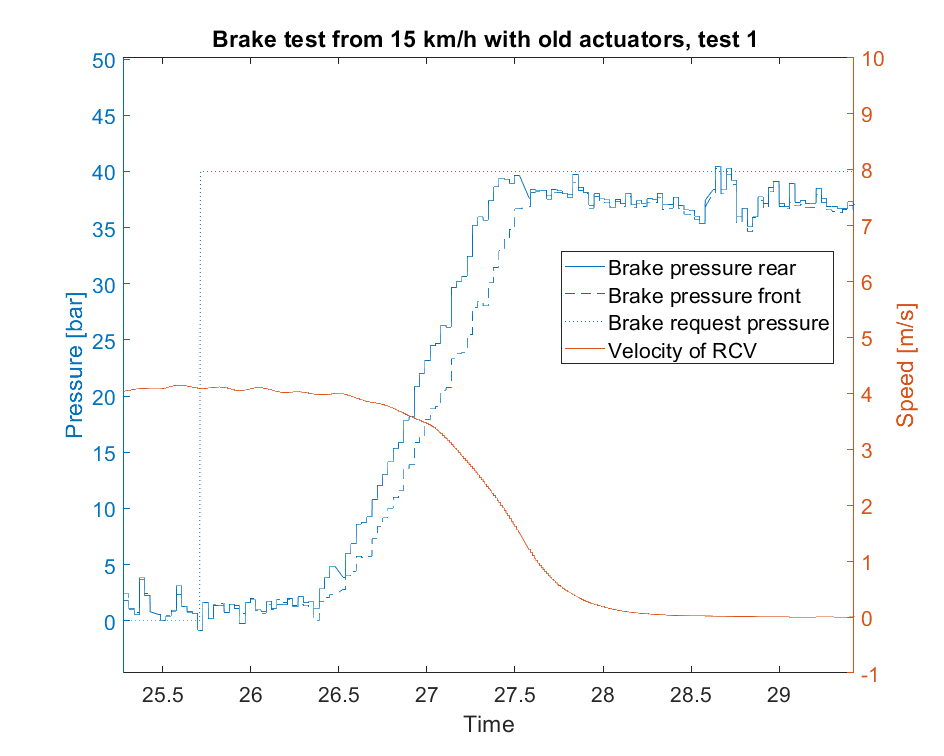
\includegraphics[width=0.8\textwidth]{Old_15kph_test1}
\caption{Old actuator, 15 km/h, test 1}
\label{fig:Old_15kph_test1}
\end{figure}

\begin{figure}[h]
\centering
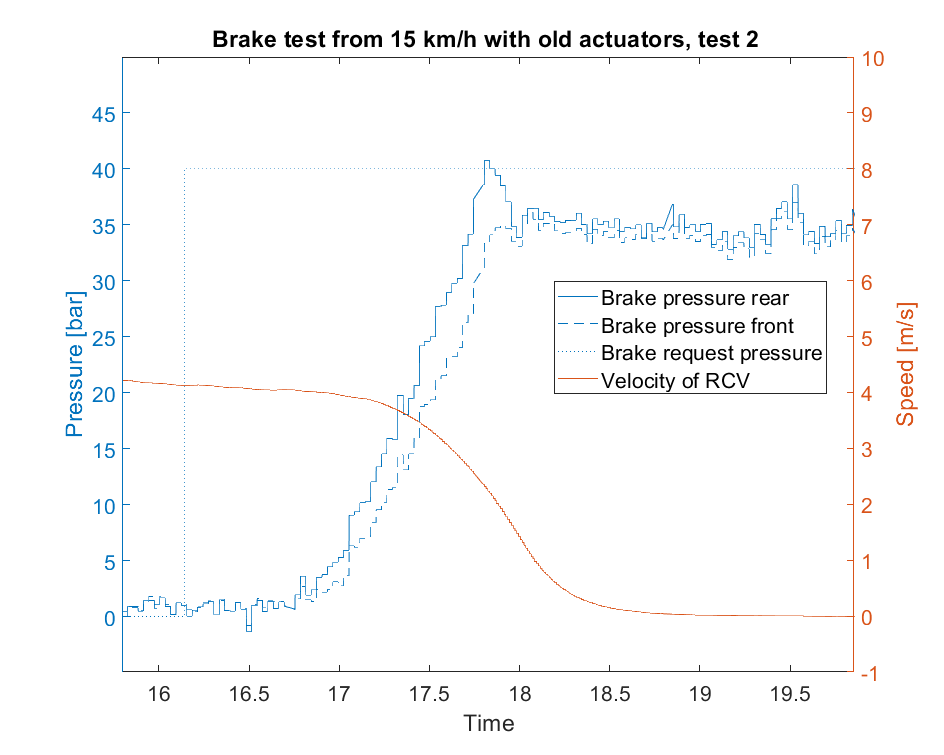
\includegraphics[width=0.8\textwidth]{Old_15kph_test2}
\caption{Old actuator, 15 km/h, test 2}
\label{fig:Old_15kph_test2}
\end{figure}

\begin{figure}[h]
\centering
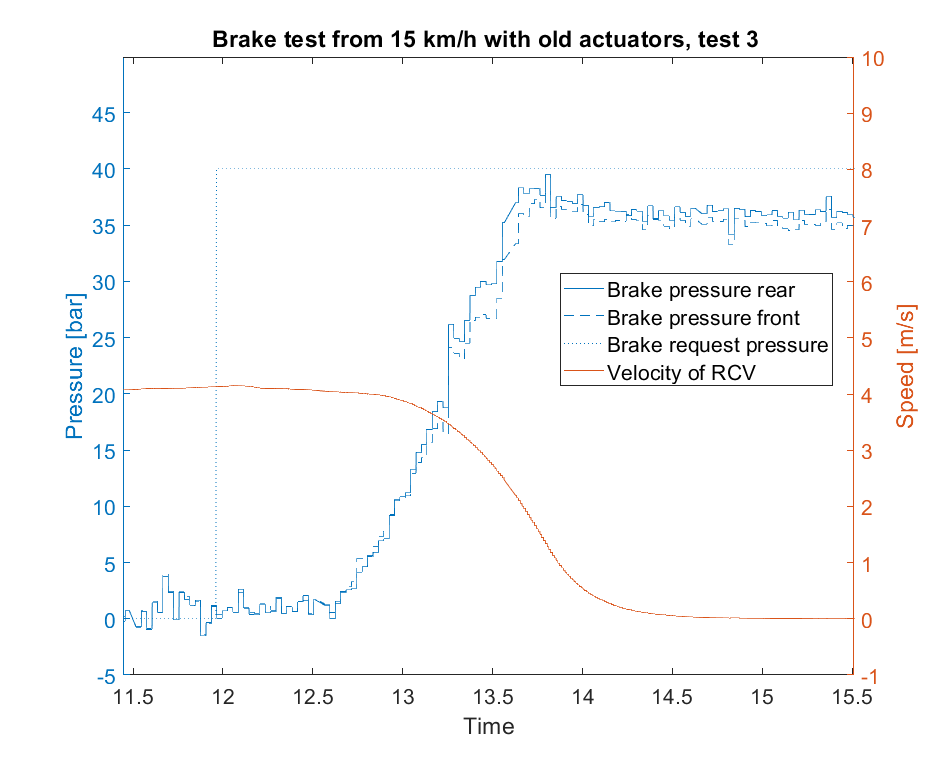
\includegraphics[width=0.8\textwidth]{Old_15kph_test3}
\caption{Old actuator, 15 km/h, test 3}
\label{fig:Old_15kph_test3}
\end{figure}

\begin{figure}[h]
\centering
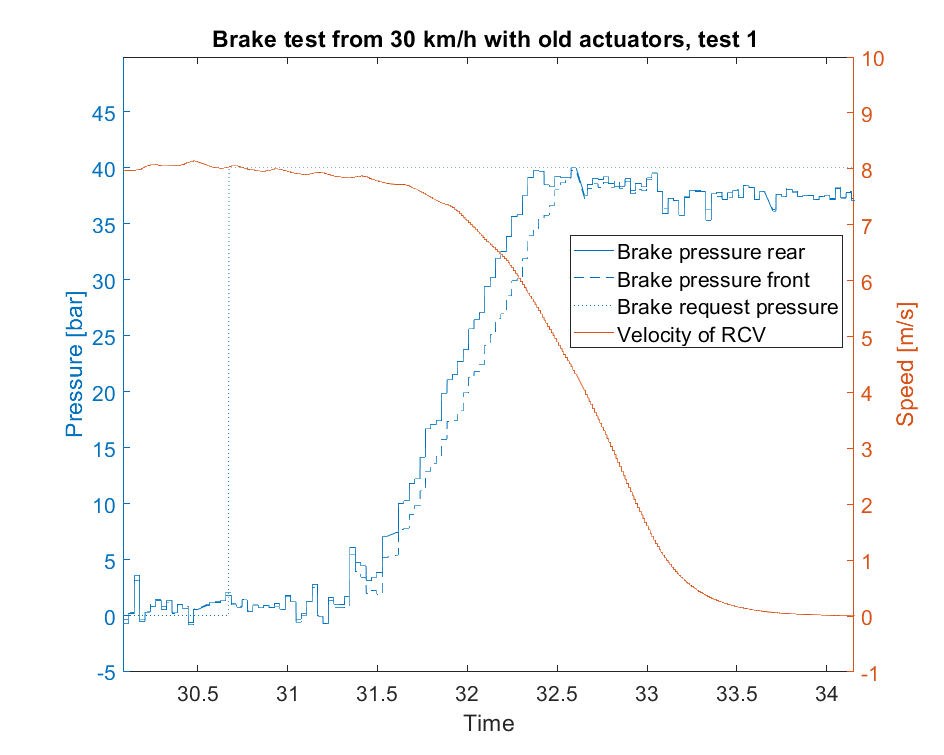
\includegraphics[width=0.8\textwidth]{Old_30kph_test1}
\caption{Old actuator, 30 km/h, test 1}
\label{fig:Old_30kph_test1}
\end{figure}

\begin{figure}[h]
\centering
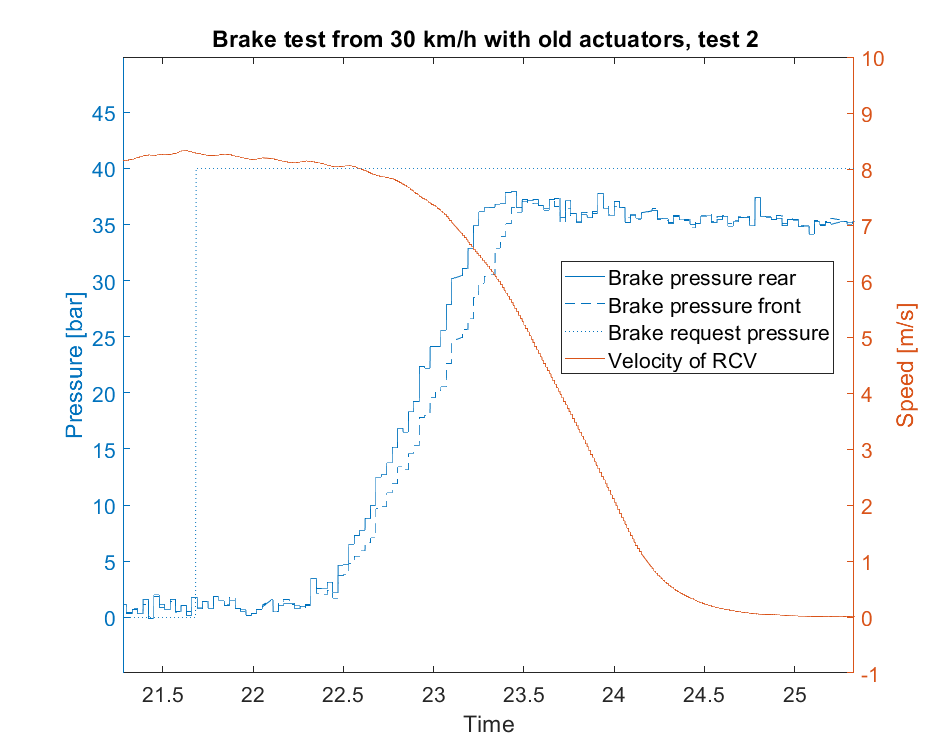
\includegraphics[width=0.8\textwidth]{Old_30kph_test2}
\caption{Old actuator, 30 km/h, test 2}
\label{fig:Old_30kph_test2}
\end{figure}

\begin{figure}[h]
\centering
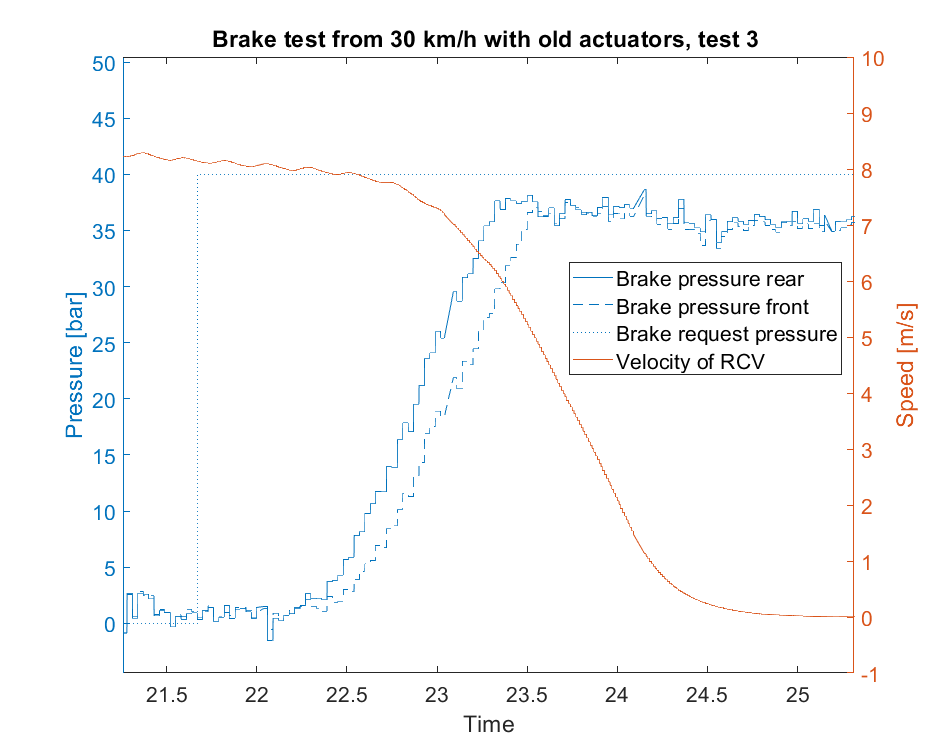
\includegraphics[width=0.8\textwidth]{Old_30kph_test3}
\caption{Old actuator, 30 km/h, test 3}
\label{fig:Old_30kph_test3}
\end{figure}

\begin{table}[hp]
  \begin{center}
    \caption{Stopping distance with both new and old actuators tested from two different speeds.}
    \label{tab:table1}
    \begin{tabular}{  c | c | c | c } % <- Alignments: columns centered, with vertical lines in between
      \textbf{Test} & \textbf{Actuator} & \textbf{Driving speed}& \textbf{Stopping distance}\\
      no. &   & [km/h] & [m] \\
      \hline
      1 & New & 15 & 3.5 \\
      2 & New & 15 & 3,2 \\
      3 & New & 15 & 3,4 \\
      \hline
      4 & New & 30 & 9,8 \\
      5 & New & 30 & 9,4 \\
      6 & New & 30 & 9,1 \\
      \hline
      7 & Old & 15 & 6,5 \\
      8 & Old & 15 & 6,6 \\
      9 & Old & 15 & 6,4 \\
      \hline
      10 & Old & 30 & 14,7 \\
      11 & Old & 30 & 15,2 \\
      12 & Old & 30 & 15,2 \\
      
    \end{tabular}
  \end{center}
\end{table}




%%%%%%%%%%%%%%%   CONCLUSION   %%%%%%%%%%%%%%%%%%

\chapter{Conclusion}
This is what a chapter looks like.
%%%%%%%%%%%%%%%   DISCUSSION   %%%%%%%%%%%%%%%%%%

\chapter{Discussion}
This is what a chapter looks like.
%%%%%%%%%%%%%%%   FUTURE WORK   %%%%%%%%%%%%%%%%%
\chapter{Future work}
This is what a chapter looks like.
(Maxtryck är 15 Bar- upplösning på sensor är 100 bar, kan bytas mot mindre och exaktare)

%%%%%%%%%%%%%%%   REFERENCES   %%%%%%%%%%%%%%%%%%

\bibliography{mybib}
%%%%%%%%%%%%%%%   APPENDIX   %%%%%%%%%%%%%%%%%%%
\glsaddall

\appendix
\addappheadtotoc
\chapter{Max Jac Datasheet}
\label{appendix:Max_Jac}
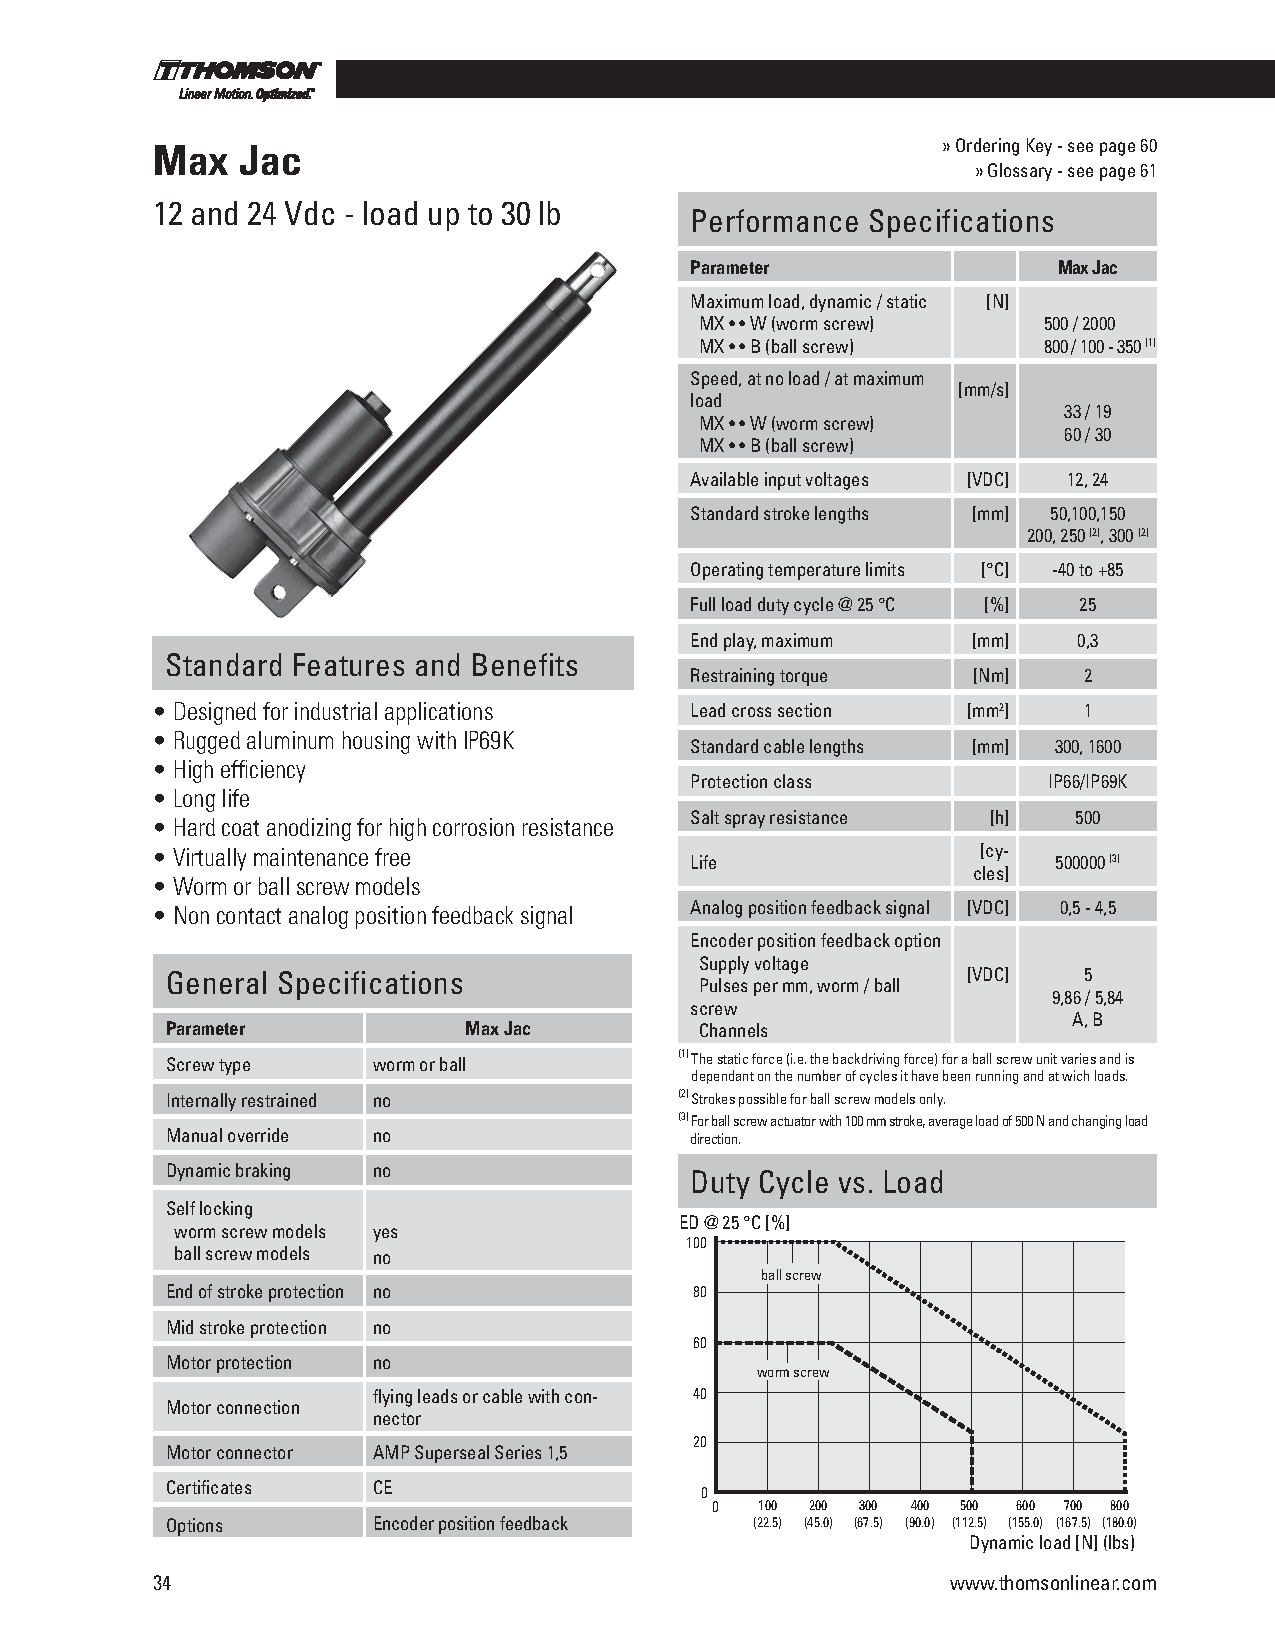
\includepdf[pages={1-2}]{Max_Jac.pdf}
\chapter{Elektrak 1 datasheet}
\label{appendix:Electrak_1}
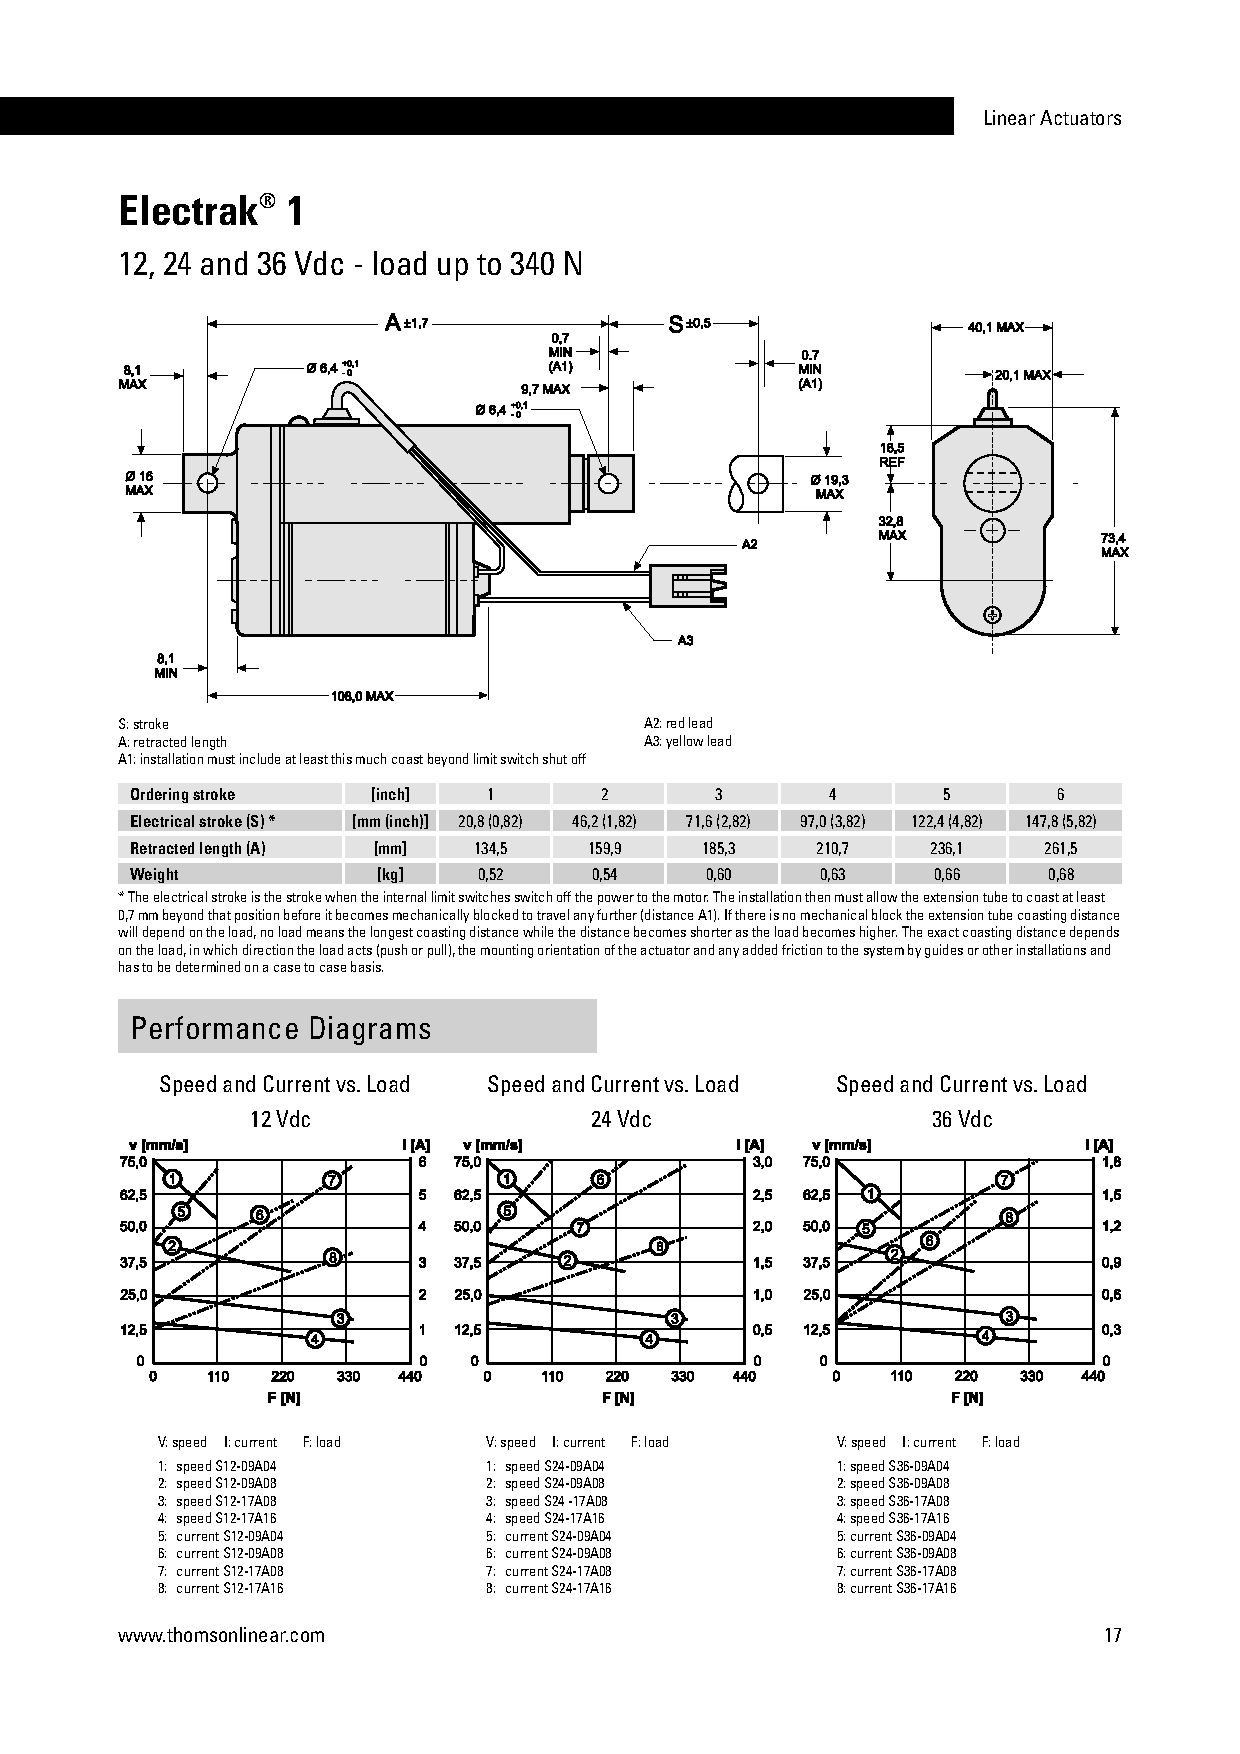
\includepdf[pages={1-2}]{Electrac_1.pdf}

\end{document}